\section{Method}
\label{sec:method}

\begin{figure*}[t]
\centering
\vspace{-18pt}
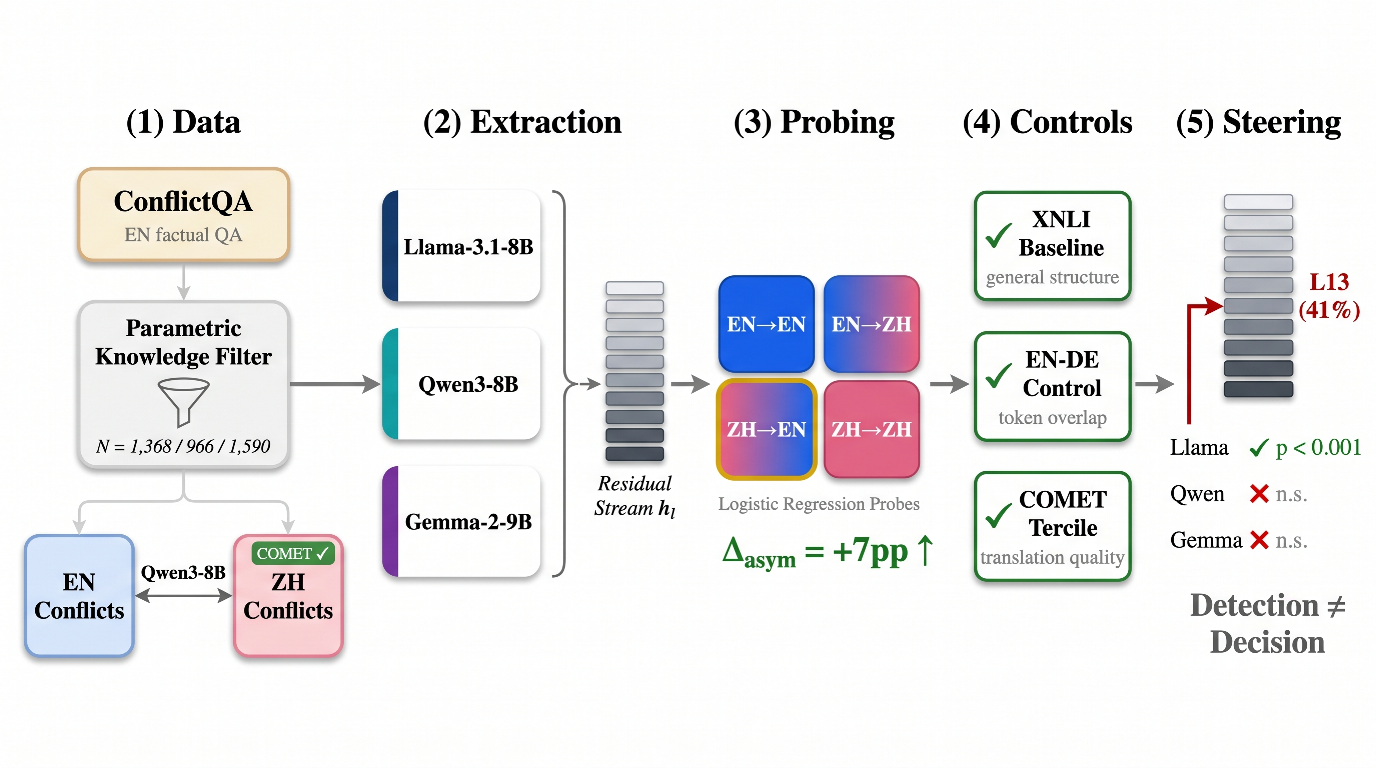
\includegraphics[width=0.88\textwidth]{fig2_pipeline.pdf}
\vspace{-14pt}
\caption{Method overview. We construct parallel EN/ZH conflict data from ConflictQA with COMET-validated translations, extract per-layer residual stream representations, train logistic regression probes in four transfer directions (EN$\to$EN, ZH$\to$ZH, EN$\to$ZH, ZH$\to$EN), and apply confound exclusion controls before causal steering validation.}
\label{fig:pipeline}
\vspace{-20pt}
\end{figure*}

Our pipeline proceeds from data construction through probing and steering (Figure~\ref{fig:pipeline}), formalized below.

\subsection{Task Formulation}
\label{sec:task}

Given a context passage $c$ and question $q$, the model produces an answer that is either \emph{contextual} (derived from $c$) or \emph{parametric} (from pre-trained knowledge).
When $c$ contradicts parametric knowledge, the choice constitutes a knowledge conflict.
We train a logistic regression probe $f_\theta(\mathbf{h}_l) = \sigma(\mathbf{w}_l^\top \mathbf{h}_l + b_l)$ on the last-token residual stream representation $\mathbf{h}_l \in \mathbb{R}^d$ at layer $l$ to predict a binary label $y \in \{\text{contextual}, \text{parametric}\}$.

\subsection{Data Construction}
\label{sec:data}

We build on ConflictQA \citep{xie2024adaptive}, which pairs questions with context passages contradicting the model's parametric knowledge.
We filter samples by querying each model without context and retaining only those answered correctly, yielding 1{,}368 samples for Llama \citep{grattafiori2024llama}, 966 for Qwen \citep{yang2025qwen3}, and 1{,}590 for Gemma \citep{team2024gemma} (80/20 train/test split with stratification).
For cross-lingual transfer, we translate all inputs into Chinese using a Qwen3-8B pipeline, with quality validated by COMET (Crosslingual Optimized Metric for Evaluation of Translation; \citet{rei2020comet}) back-translation scores used in confound analysis (\S\ref{sec:confound_method}).

\subsection{Activation Extraction and Probing}
\label{sec:extraction}

For each input, we construct English and Chinese versions and extract the last-token residual stream $\mathbf{h}_l \in \mathbb{R}^d$ at every layer $l$ ($L = 32$ for Llama, $36$ for Qwen, $42$ for Gemma; $d = 4096$ for Llama/Qwen, $3584$ for Gemma), following the last-token aggregation principle \citep{belinkov2022probing}.
We record the model's answer and assign binary labels (contextual vs.\ parametric).

\label{sec:probing}
At each layer, we train an $L_2$-regularized logistic regression probe ($C = 1.0$; \citealt{belinkov2022probing, hewitt2019designing}) and evaluate with balanced accuracy to account for class imbalance (contextual/parametric ratios range from 40/60 to 55/45 across models).
We report peak-layer accuracy (maximum across layers) as the primary metric.
To verify that probes capture conflict-specific structure rather than arbitrary linear separability, we run a selectivity control \citep{hewitt2019designing}: probes trained on permuted labels should yield chance-level accuracy if the original signal is meaningful.
As a complementary analysis, we train two-layer multilayer perceptron (MLP) probes (hidden dimension 256, ReLU activation, same $L_2$ penalty) to test whether conflict information is encoded non-linearly at layers where linear probes underperform.
Confidence intervals are estimated via bootstrap resampling ($n = 2{,}000$) \citep{ulmer2022deep}.

\subsection{Cross-Lingual Transfer Protocol}
\label{sec:transfer}

We evaluate probes in four directions: EN$\to$EN, ZH$\to$ZH (within-language upper bounds), EN$\to$ZH, and ZH$\to$EN (cross-lingual transfer).
We quantify directional asymmetry as $\Delta_{\text{asym}} = \text{acc}(\text{ZH}{\to}\text{EN}) - \text{acc}(\text{EN}{\to}\text{ZH})$, computed via paired bootstrap (same resampled indices for both directions).

\subsection{Confound Exclusion}
\label{sec:confound_method}

We exclude two artifacts: (1)~\emph{translation quality}, where we stratify test samples by COMET score into terciles and compare probe accuracy (Fisher's exact test); (2)~\emph{token overlap}, where we compute per-sample Jaccard similarity between English and Chinese token sets and test for correlation with accuracy (Pearson's $r$).
As a typological control, we additionally translate samples into German (EN$\to$DE) using the same pipeline; since German shares substantially more lexical overlap with English than Chinese does, a positive EN-DE asymmetry would implicate shared tokens rather than cross-lingual structure.
As a \emph{non-conflict baseline}, we apply the same probing pipeline to XNLI entailment-versus-contradiction \citep{conneau2018xnli}; if $\Delta_{\text{asym}} > 0$ also appears in this non-conflict task, the asymmetry reflects a general cross-lingual property rather than conflict-specific encoding.

\subsection{Representation Steering}
\label{sec:steering_method}

To test whether the probe direction is causally relevant \citep{hewitt2019designing}, we inject $\alpha \cdot \mathbf{w}_l$ (the probe weight vector from \S\ref{sec:task}) into the last-token residual stream at layer $l$ during inference \citep{li2023iti, zou2023representation}:
$\mathbf{h}'_l = \mathbf{h}_l + \alpha \cdot \mathbf{w}_l$,
where positive $\alpha$ pushes toward the contextual direction and negative toward the parametric.
As control, we inject a random vector $\mathbf{r} \sim \mathcal{N}(\mathbf{0}, \mathbf{I})$, normalized to $\|\mathbf{r}\| = \|\mathbf{w}_l\|$, at the same layer and position; the random control isolates the effect of direction from magnitude.
We also test an all-position variant where the perturbation is applied to every token position (not just the last token) to determine whether the causal signal is position-specific.
We measure the flip rate (fraction of samples switching answer category) and compare via Fisher's exact test.
We apply Bonferroni correction per layer ($k = 10$ $\alpha$ values), treating each layer as an independent hypothesis about causal locus, consistent with prior work in mechanistic interpretability that tests layers individually \citep{meng2022locating, geiger2024finding}.
For Llama L13 (the layer showing causal effects), this yields a corrected threshold of $0.05/10 = 0.005$.
For last-token injection, we sweep $\alpha \in \{\pm 20, \pm 10, \pm 5, \pm 2, \pm 1\}$ ($k = 10$) at three Llama layers (L13, L18, L28) spanning 41--88\% depth; all-position and cross-model experiments use a reduced 6-value grid ($\alpha \in \{\pm 20, \pm 10, \pm 5\}$).
Steering evaluation uses only the conflict-condition subset of the English test data, yielding $n_{\text{test}}$ smaller than the full probe test set (e.g., 136 vs.\ 272 for Llama).